\chapter{Classical Yang-Mills Theory and Matter Fields}
\label{ch:vol2-classical-yang-mills-matter}

\section{Local Gauge Fields}

This chapter formulates the local classical field theory of nonabelian gauge
fields.  We work first on a spacetime region over which the relevant principal
\(G\)-bundle has been trivialized.  In such a local trivialization, a gauge
field is represented by a Hermitian matrix-valued one-form
\[
  A=A_\mu(x)\,\dd x^\mu,
  \qquad
  A_\mu(x)=A^a_\mu(x)t^a .
\]
The index \(\mu=0,\ldots,D-1\) is a spacetime index.  The index \(a\) labels a
basis of the gauge algebra in the Hermitian-generator convention.  If
\(\mathfrak g_{\mathrm{ah}}=\operatorname{Lie}(G)\) is realized by
anti-Hermitian matrices in a unitary representation, then the Hermitian
generators used here span \(i\,\mathfrak g_{\mathrm{ah}}\).  The associated
anti-Hermitian connection one-form, denoted \(\mathsf A_{\mathrm{ah}}\), is
\(\mathsf A_{\mathrm{ah}}=-\ii A\).  We write
\(\mathfrak g:=i\,\mathfrak g_{\mathrm{ah}}\) for this Hermitian coordinate
space.  Throughout this chapter \([X,Y]\) denotes the ordinary matrix
commutator of Hermitian representatives, while the real compact Lie bracket in
Hermitian coordinates is
\[
  [X,Y]_{\mathrm H}:=-\ii[X,Y].
\]
With this convention,
\begin{equation}
  [t^a,t^b]=\ii f^{ab}{}_{c}t^c .
  \label{eq:ym-lie-algebra-conventions}
\end{equation}
The real constants \(f^{ab}{}_{c}\) are the structure constants of
\([\ ,\ ]_{\mathrm H}\) in this basis.  Formulas below include explicit factors
of \(\ii\) so that \(A_\mu\), \(\zeta\), and \(F_{\mu\nu}\) remain Hermitian
matrix fields.

The infinitesimal local transformation with parameter
\(\zeta(x)=\zeta_a(x)t^a\) is
\begin{equation}
  \delta_\zeta A_\mu
  =
  \partial_\mu\zeta-\ii[A_\mu,\zeta].
  \label{eq:ym-infinitesimal-gauge-transformation}
\end{equation}
In components,
\begin{equation}
  \delta_\zeta A^a_\mu
  =
  \partial_\mu\zeta^a+f^{bc}{}_{a}A^b_\mu\zeta^c,
  \label{eq:ym-infinitesimal-component-transformation}
\end{equation}
with indices raised or lowered by the invariant quadratic form introduced
below.  The derivative term records the freedom to change local trivialization
from point to point, while the commutator term records the adjoint action of
the Lie algebra on itself.

\begin{figure}[H]
  \centering
  \resizebox{0.96\textwidth}{!}{%
  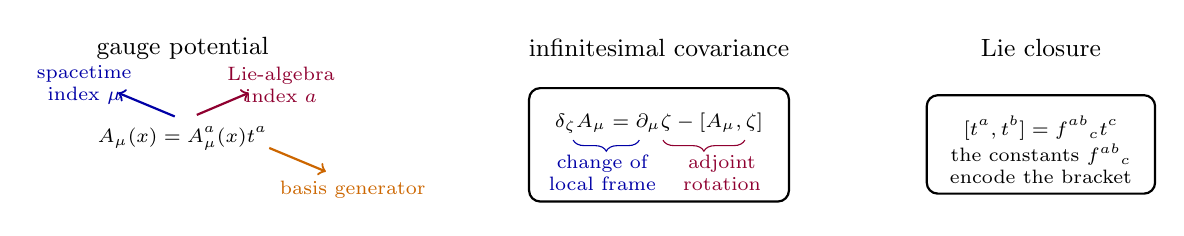
\begin{tikzpicture}[x=1cm,y=1cm,every node/.style={font=\scriptsize}]
    \node[font=\small] at (0,2.35) {gauge potential};
    \node at (0,1.20) {\(\displaystyle A_\mu(x)=A^a_\mu(x)t^a\)};
    \draw[blue!65!black,->,thick] (-0.10,1.48)--(-0.82,1.78);
    \node[blue!65!black,align=center] at (-1.25,1.88)
      {spacetime\\index \(\mu\)};
    \draw[purple!75!black,->,thick] (0.18,1.50)--(0.84,1.78);
    \node[purple!75!black,align=center] at (1.25,1.88)
      {Lie-algebra\\index \(a\)};
    \draw[orange!80!black,->,thick] (1.10,1.08)--(1.82,0.78);
    \node[orange!80!black,align=center] at (2.16,0.55)
      {basis generator};

    \begin{scope}[shift={(4.4,0)}]
      \node[font=\small] at (1.65,2.35) {infinitesimal covariance};
      \draw[rounded corners=4pt,thick] (0,0.40) rectangle (3.30,1.84);
      \node at (1.65,1.40)
        {\(\displaystyle
        \delta_\zeta A_\mu=\partial_\mu\zeta-\ii[A_\mu,\zeta]\)};
      \node[align=center,blue!65!black] at (0.93,0.76)
        {change of\\local frame};
      \node[align=center,purple!75!black] at (2.45,0.76)
        {adjoint\\rotation};
      \draw[blue!65!black,decorate,decoration={brace,mirror,amplitude=4pt}]
        (0.56,1.18)--(1.40,1.18);
      \draw[purple!75!black,decorate,decoration={brace,mirror,amplitude=4pt}]
        (1.70,1.18)--(2.74,1.18);
    \end{scope}

    \begin{scope}[shift={(9.45,0)}]
      \node[font=\small] at (1.45,2.35) {Lie closure};
      \draw[rounded corners=4pt,thick] (0.0,0.50) rectangle (2.90,1.75);
      \node at (1.45,1.33)
        {\(\displaystyle [t^a,t^b]=\ii f^{ab}{}_{c}t^c\)};
      \node[align=center] at (1.45,0.88)
        {the constants \(f^{ab}{}_{c}\)\\encode the bracket};
    \end{scope}
  \end{tikzpicture}
  }
  \caption{The local gauge field carries a spacetime vector index and a
  Lie-algebra index.  The infinitesimal transformation combines the derivative
  of the local parameter with the adjoint action of the Lie algebra.}
  \label{fig:ym-index-and-infinitesimal-data}
\end{figure}

The finite transformation is most cleanly stated using a smooth
\(G\)-valued function \(g(x)\).  With
\[
  g(x)=\exp\{\ii\zeta_a(x)t^a\},
\]
define
\begin{equation}
  A_\mu'
  =
  gA_\mu g^{-1}+\ii g\,\partial_\mu g^{-1}.
  \label{eq:ym-finite-gauge-transformation}
\end{equation}
The Baker-Campbell-Hausdorff formula
\[
  \log(\ee^X\ee^Y)
  =
  X+Y+\frac12[X,Y]
  +\frac1{12}[X,[X,Y]]
  -\frac1{12}[Y,[X,Y]]+\cdots
\]
shows how products of exponentials are controlled by the Lie bracket.  The
identity
\[
  \ee^X Y\ee^{-X}
  =
  Y+[X,Y]+\frac1{2!}[X,[X,Y]]+\cdots
\]
then shows that conjugation by \(g(x)\) maps \(\mathfrak g\) to
\(\mathfrak g\).  Thus \eqref{eq:ym-finite-gauge-transformation} produces
another local representative \(A_\mu'=A_\mu^{\prime a}t^a\).

The same formula is also the transition law between local trivializations.
If \(U_i\) and \(U_j\) are two coordinate patches and
\(h_{ji}:U_i\cap U_j\to G\) is the transition function, then their local
connection representatives satisfy
\[
  A_\mu^{(j)}
  =
  h_{ji}A_\mu^{(i)}h_{ji}^{-1}
  +\ii h_{ji}\partial_\mu h_{ji}^{-1}.
\]
Thus the local field \(A_\mu\) is not itself a globally defined tensor on a
nontrivial bundle.  The curvature constructed below does glue covariantly:
\[
  F_{\mu\nu}^{(j)}=h_{ji}F_{\mu\nu}^{(i)}h_{ji}^{-1}.
\]
The local formulas therefore describe a connection on a principal bundle; they
do not assume that the bundle is globally trivial.

\section{Curvature and the Yang-Mills Action}

Define the covariant differential operator
\begin{equation}
  \nabla_\mu:=\partial_\mu-\ii A_\mu .
  \label{eq:ym-adjoint-covariant-operator}
\end{equation}
The gauge coupling has been absorbed into the connection in this chapter:
relative to the QED convention \(\partial_\mu-\ii g A_\mu\), the present
connection is \(A_\mu^{\rm here}=gA_\mu^{\rm QED}\).  With this choice the
curvature and the action carry the coupling in the Yang--Mills kinetic term
rather than in the covariant derivative.
The finite transformation law \eqref{eq:ym-finite-gauge-transformation} is
equivalent to
\begin{equation}
  \nabla_\mu'=g\nabla_\mu g^{-1},
  \label{eq:ym-covariant-operator-transformation}
\end{equation}
where the factors are multiplied as differential operators.  The curvature is
\begin{equation}
  F_{\mu\nu}
  :=
  \ii[\nabla_\mu,\nabla_\nu]
  =
  \partial_\mu A_\nu-\partial_\nu A_\mu-\ii[A_\mu,A_\nu]
  =
  F^a_{\mu\nu}t^a .
  \label{eq:ym-field-strength-definition}
\end{equation}
It follows from \eqref{eq:ym-covariant-operator-transformation} that
\begin{equation}
  F'_{\mu\nu}=gF_{\mu\nu}g^{-1}.
  \label{eq:ym-curvature-covariance}
\end{equation}

\begin{figure}[H]
  \centering
  \resizebox{0.96\textwidth}{!}{%
  \begin{tikzpicture}[x=1cm,y=1cm,every node/.style={font=\scriptsize}]
    \node[font=\small] at (0,2.55) {connection};
    \draw[rounded corners=4pt,thick] (-1.5,0.65) rectangle (1.5,1.75);
    \node at (0,1.20) {\(\nabla_\mu=\partial_\mu-\ii A_\mu\)};

    \draw[-{Latex[length=2mm]},thick] (1.75,1.20)--(3.05,1.20);
    \node[align=center] at (2.40,1.60) {commutator};

    \node[font=\small] at (4.55,2.55) {curvature};
    \draw[rounded corners=4pt,thick] (3.10,0.65) rectangle (5.95,1.75);
    \node at (4.53,1.20) {\(F_{\mu\nu}=\ii[\nabla_\mu,\nabla_\nu]\)};

    \draw[-{Latex[length=2mm]},thick] (6.18,1.20)--(7.45,1.20);
    \node[align=center] at (6.82,1.60) {invariant\\trace};

    \node[font=\small] at (9.05,2.55) {action density};
    \draw[rounded corners=4pt,thick] (7.55,0.65) rectangle (10.55,1.75);
    \node at (9.05,1.20)
      {\(\displaystyle -\frac1{2g_{\mathrm{YM}}^2}\operatorname{tr}(F_{\mu\nu}F^{\mu\nu})\)};

    \draw[purple!75!black,thick,-{Latex[length=2mm]}]
      (0,0.45) .. controls (1.6,-0.55) and (3.2,-0.55) .. (4.55,0.45);
    \node[purple!75!black,align=center] at (2.35,-0.78)
      {\(\nabla_\mu'=g\nabla_\mu g^{-1}\) implies
      \(F_{\mu\nu}'=gF_{\mu\nu}g^{-1}\)};
    \node[blue!65!black,align=center] at (9.05,-0.50)
      {cyclicity removes the conjugation};
  \end{tikzpicture}
  }
  \caption{The Yang-Mills field strength is the curvature of the covariant
  differential operator.  Its conjugation law is converted into a gauge-invariant
  action density by an invariant trace.}
  \label{fig:ym-curvature-action-chain}
\end{figure}

An invariant trace is a symmetric bilinear form on \(\mathfrak g\), written in
a chosen representation as
\begin{equation}
  \operatorname{tr}(t^a t^b)=\kappa^{ab}.
  \label{eq:ym-trace-kappa}
\end{equation}
Cyclicity gives
\[
  \operatorname{tr}([t^a,t^b]t^c)
  =
  \operatorname{tr}(t^a[t^b,t^c])
\]
and, equivalently,
\[
  \operatorname{tr}(gXg^{-1}gYg^{-1})
  =
  \operatorname{tr}(XY)
\]
for Lie-algebra-valued \(X,Y\).  It also gives the invariant tensor
\begin{equation}
  f^{abc}:=f^{ab}{}_{e}\kappa^{ec}
  =
  -\ii\,\operatorname{tr}([t^a,t^b]t^c),
  \label{eq:ym-fabc-lowered}
\end{equation}
which is completely antisymmetric in \(a,b,c\).

The Lorentzian Yang-Mills Lagrangian density is
\begin{equation}
  \mathcal L_{\mathrm{YM}}
  =
  -\frac1{2g_{\mathrm{YM}}^2}
  \operatorname{tr}(F_{\mu\nu}F^{\mu\nu}).
  \label{eq:ym-lagrangian-density}
\end{equation}
If \(\operatorname{tr}(t^a t^b)=\frac12\delta^{ab}\), this is
\[
  \mathcal L_{\mathrm{YM}}
  =
  -\frac1{4g_{\mathrm{YM}}^2}F^a_{\mu\nu}F^{a\mu\nu}.
\]
For a unitary Lorentzian quantum theory built from these fields, the invariant
quadratic form on the gauge algebra is chosen positive definite.  Equivalently,
the local gauge algebra is a compact reductive Lie algebra: a direct sum of
abelian \(\mathbb R\) factors and compact simple factors.  The compact simple
factors are the simple Lie algebras of Cartan type
\[
  A,\ B,\ C,\ D,\ E,\ F,\ G .
\]
For these algebras one may choose a linear basis in which
\[
  \kappa^{ab}=\operatorname{tr}(t^a t^b)=\frac12\delta^{ab},
\]
which is the normalization used unless another normalization is explicitly
declared.

The basic example \(SU(2)\) has
\[
  t^a=\frac12\sigma^a,\qquad a=1,2,3,
\]
where \(\sigma^a\) are the Pauli matrices.  More generally,
the Hermitian coordinate space \(i\,\mathfrak{su}(N)\) is represented by
traceless Hermitian \(N\times N\) matrices, and
\[
  SU(N)=\{g\in U(N):\det g=1\}.
\]

In four spacetime dimensions there is another local gauge-invariant Lorentz
scalar of power-counting dimension four, written in the trace convention just
fixed.\footnote{With \(F_{\mu\nu}=F^a_{\mu\nu}t^a\) and
\(\operatorname{tr}(t^at^b)=\frac12\delta^{ab}\),
\(\operatorname{tr}(F_{\mu\nu}F_{\rho\sigma})
=\frac12F^a_{\mu\nu}F^a_{\rho\sigma}\).  Component formulas written with
\(\operatorname{tr}(t^at^b)=\delta^{ab}\) therefore differ by this factor
of \(2\).}
\begin{equation}
  \Delta\mathcal L_\theta
  =
  \frac{\theta}{32\pi^2}
  \epsilon^{\mu\nu\rho\sigma}
  \operatorname{tr}(F_{\mu\nu}F_{\rho\sigma}).
  \label{eq:ym-theta-density}
\end{equation}
With \(\operatorname{tr}(t^at^b)=\frac12\delta^{ab}\), this equals
\[
  \frac{\theta}{64\pi^2}
  \epsilon^{\mu\nu\rho\sigma}F^a_{\mu\nu}F^a_{\rho\sigma}.
\]
Authors who write the component density with coefficient
\(\theta/(32\pi^2)\) are using a trace convention without the factor
\(\frac12\), or are absorbing that factor into the definition of the component
curvature.
This density is odd under parity and time reversal.  In local coordinates it
is a total derivative, so it does not change the local Euler-Lagrange equations
under boundary conditions that keep the boundary variation fixed.  Perturbation
theory around the trivial gauge-field sector consequently has no local Feynman
vertex associated with \eqref{eq:ym-theta-density}.  Finite-action gauge fields
may approach nontrivial pure gauges at spatial infinity, and then the spacetime
integral of \eqref{eq:ym-theta-density} can be nonzero.  Thus \(\theta\)
enters through global topological sectors of the gauge field.

\section{Matter Representations}

Let \(R\) be a finite-dimensional representation of \(G\) on a vector space
\(V_R\).  The matter fields below use complex \(V_R\); real representations,
such as the adjoint representation, are included by complexification when they
are compared with complex representations.  The representation is a
homomorphism
\begin{equation}
  \rho_R:G\longrightarrow GL(V_R),
  \qquad
  \rho_R(gh)=\rho_R(g)\rho_R(h).
  \label{eq:ym-group-representation}
\end{equation}
Its derived Lie-algebra representation is the linear map
\(\widetilde\rho_R:\mathfrak g\to\operatorname{End}(V_R)\) determined by
\begin{equation}
  \rho_R(\ee^{\ii\zeta_a t^a})
  =
  \ee^{\ii\zeta_a t_R^a},
  \qquad
  t_R^a:=\widetilde\rho_R(t^a).
  \label{eq:ym-lie-algebra-representation}
\end{equation}
The matrices \(t_R^a\) obey
\begin{equation}
  [t_R^a,t_R^b]=\ii f^{ab}{}_{c}t_R^c.
  \label{eq:ym-representation-commutator}
\end{equation}
For compact \(G\), every finite-dimensional complex representation used in a
unitary theory may be equipped with a \(G\)-invariant Hermitian inner product.
In such a basis the matrices \(t_R^a\) are Hermitian.  This is the matter-field
version of the same Hermitian convention used for the gauge potential.

For \(G=SU(N)\), three representations recur throughout gauge theory:
\[
\begin{array}{c|c|c}
\text{representation} & V_R & \text{infinitesimal generators} \\ \hline
\text{fundamental } \square & \mathbb C^N & t_\square^a=t^a \\
\text{anti-fundamental } \overline{\square} & \mathbb C^N &
  t_{\overline{\square}}^a=-(t^a)^* \\
\text{adjoint} & \mathfrak g_{\mathbb C} &
  t_{\mathrm{adj}}^a(t^b)=\ii f^{ab}{}_{c}t^c
\end{array}
\]
In the fundamental representation,
\(\rho_{\square}(g)=g\) and \(t_{\square}^a=t^a\).  In the
anti-fundamental representation,
\[
  \rho_{\overline{\square}}(g)=g^*
  \qquad\hbox{complex conjugation, without transposition,}
\]
so differentiating
\(\rho_{\overline{\square}}(\ee^{\ii\zeta_a t^a})
=\ee^{\ii\zeta_a t_{\overline{\square}}^a}\) gives
\(t_{\overline{\square}}^a=-(t^a)^*\).
Here \(\mathfrak g_{\mathbb C}\) denotes the complexification of the real
Hermitian coordinate space.  A real adjoint-valued field is obtained by
imposing the corresponding reality condition on its components.  The finite
adjoint representation is conjugation on the algebra:
\[
  v\mapsto gvg^{-1},
  \qquad
  \rho_{\mathrm{adj}}(g)v=gvg^{-1}.
\]
Its infinitesimal form is consistent with the convention
differentiating \(v\mapsto \ee^{\ii\zeta_a t^a}v\ee^{-\ii\zeta_a t^a}\):
\[
  \delta v
  =
  \ii\zeta_a[t^a,v]
  =
  \ii\zeta_a t_{\mathrm{adj}}^a v .
\]

\begin{figure}[H]
  \centering
  \resizebox{0.96\textwidth}{!}{%
  \begin{tikzpicture}[x=1cm,y=1cm,every node/.style={font=\scriptsize}]
    \node[font=\small] at (0,3.05) {\(SU(N)\) representation data};

    \draw[rounded corners=4pt,thick] (-5.90,0.35) rectangle (-2.10,2.50);
    \node[font=\bfseries] at (-4.00,2.17) {fundamental \(\square\)};
    \node at (-4.00,1.67) {\(V=\mathbb C^N\)};
    \node at (-4.00,1.25) {\(\rho_\square(g)=g\)};
    \node at (-4.00,0.83) {\(t_\square^a=t^a\)};

    \draw[rounded corners=4pt,thick] (-1.90,0.35) rectangle (1.90,2.50);
    \node[font=\bfseries\small] at (0,2.17)
      {anti-fundamental \(\overline{\square}\)};
    \node at (0,1.67) {\(V=\mathbb C^N\)};
    \node at (0,1.25) {\(\rho_{\overline{\square}}(g)=g^*\)};
    \node at (0,0.83) {\(t_{\overline{\square}}^a=-(t^a)^*\)};

    \draw[rounded corners=4pt,thick] (2.10,0.35) rectangle (5.90,2.50);
    \node[font=\bfseries] at (4.00,2.17) {adjoint};
    \node at (4.00,1.67) {\(V=\mathfrak g\) or \(\mathfrak g_{\mathbb C}\)};
    \node at (4.00,1.25) {\(\rho_{\mathrm{adj}}(g)v=gvg^{-1}\)};
    \node at (4.00,0.83) {\((t_{\mathrm{adj}}^a)^b{}_{c}=\ii f^{ab}{}_{c}\)};

    \node[font=\small] at (0,-0.10) {QCD quark indices};
    \draw[rounded corners=4pt,thick] (-3.60,-1.95) rectangle (3.60,-0.45);
    \node at (0,-0.92)
      {\(\psi^{\,i}_{I\alpha}(x)\)};
    \node[blue!65!black,align=center] at (-2.22,-1.47)
      {\(i=1,\ldots,N\)\\color in \(\square\)};
    \node[purple!75!black,align=center] at (0,-1.47)
      {\(I=1,\ldots,N_f\)\\flavor};
    \node[orange!80!black,align=center] at (2.22,-1.47)
      {\(\alpha\)\\spinor};
  \end{tikzpicture}
  }
  \caption{The fundamental, anti-fundamental, and adjoint representations of
  \(SU(N)\) used in Yang-Mills theory and QCD.  The anti-fundamental finite
  action is complex conjugation of the matrix entries, not Hermitian
  conjugation.}
  \label{fig:ym-su-n-representation-data}
\end{figure}

If \(\psi(x)\in V_R\), its finite gauge transformation is
\begin{equation}
  \psi'(x)=\rho_R(g(x))\psi(x).
  \label{eq:ym-matter-finite-transformation}
\end{equation}
The covariant derivative acting on \(\psi\) is
\begin{equation}
  D_\mu\psi
  =
  \partial_\mu\psi-\ii A^a_\mu t_R^a\psi.
  \label{eq:ym-matter-covariant-derivative}
\end{equation}
Using \eqref{eq:ym-finite-gauge-transformation} and
\eqref{eq:ym-group-representation}, one obtains
\begin{equation}
  (D_\mu\psi)'=\rho_R(g)D_\mu\psi.
  \label{eq:ym-matter-covariant-derivative-transform}
\end{equation}
This covariance is the algebraic reason that replacing ordinary derivatives
by \(D_\mu\) produces gauge-invariant matter kinetic terms.
For example, if \((\ ,\ )_R\) is the invariant Hermitian pairing on \(V_R\),
then \((D_\mu\psi,D^\mu\psi)_R\) is gauge invariant for scalar matter.  For
Dirac matter, the gauge index contraction in \(\bar\psi\gamma^\mu D_\mu\psi\)
uses the pairing between \(R^*\) and \(R\).  Mass and Yukawa couplings are
gauge invariant only when their flavor and representation tensors define
intertwiners from the tensor product of fields to the trivial representation.

\begin{figure}[H]
  \centering
  \resizebox{0.96\textwidth}{!}{%
  \begin{tikzpicture}[x=1cm,y=1cm,every node/.style={font=\scriptsize}]
    \node[font=\small] at (0,2.55) {matter field};
    \draw[rounded corners=4pt,thick] (-1.35,0.65) rectangle (1.35,1.75);
    \node at (0,1.22) {\(\psi(x)\in V_R\)};
    \draw[-{Latex[length=2mm]},thick] (1.55,1.22)--(3.15,1.22);
    \node[align=center] at (2.35,1.65)
      {local\\transformation};

    \draw[rounded corners=4pt,thick] (3.30,0.65) rectangle (6.10,1.75);
    \node at (4.70,1.22) {\(\psi'=\rho_R(g)\psi\)};

    \draw[-{Latex[length=2mm]},thick] (6.30,1.22)--(7.88,1.22);
    \node[align=center] at (7.08,1.65)
      {covariant\\derivative};

    \draw[rounded corners=4pt,thick] (8.05,0.65) rectangle (11.20,1.75);
    \node at (9.62,1.22)
      {\(D_\mu=\partial_\mu-\ii A^a_\mu t_R^a\)};

    \node[blue!65!black,align=center] at (4.70,0.10)
      {\(\rho_R(gh)=\rho_R(g)\rho_R(h)\)};
    \node[purple!75!black,align=center] at (9.62,0.10)
      {\((D_\mu\psi)'=\rho_R(g)D_\mu\psi\)};
  \end{tikzpicture}
  }
  \caption{A matter field transforms in a representation \(R\) of the gauge
  group.  The covariant derivative uses the corresponding Lie-algebra
  generators \(t_R^a\), so \(D_\mu\psi\) transforms in the same representation
  as \(\psi\).}
  \label{fig:ym-matter-representation-covariance}
\end{figure}

\section{QCD Notation and Chiral Masses}

For QCD with gauge group \(SU(N)\), a quark field carries three kinds of
indices:
\[
  \psi^{\,i}_{I\alpha}(x),
  \qquad
  i=1,\ldots,N,\quad
  I=1,\ldots,N_f .
\]
Here \(i\) is the color index in the fundamental representation, \(I\) is a
flavor index, and \(\alpha\) is a spinor index.  The conjugate field
\(\bar\psi\) carries the anti-fundamental color representation.

For these quarks, the local four-dimensional terms that are Poincare
invariant, gauge invariant, and power-counting renormalizable have the gauge
part
\[
  -\frac1{2g_{\mathrm{YM}}^2}\operatorname{tr}(F_{\mu\nu}F^{\mu\nu})
  +
  \frac{\theta}{32\pi^2}
  \epsilon^{\mu\nu\rho\sigma}
  \operatorname{tr}(F_{\mu\nu}F_{\rho\sigma})
\]
and the fermion part
\begin{equation}
  \mathcal L_\psi
  =
  -\bar\psi_I\gamma^\mu D_\mu\psi_I
  -
  m_{IJ}\bar\psi_I\psi_J
  -
  \widetilde m_{IJ}\bar\psi_I\gamma_5\psi_J .
  \label{eq:qcd-fermion-mass-lagrangian}
\end{equation}
The matrices \(m\) and \(\widetilde m\) act on flavor and are Hermitian in a
Hermitian Lorentzian action.

For chiral notation, use the convention fixed in
Chapter~\ref{ch:spinor-fields-fermionic-path-integrals},
\(\gamma_5=-\ii\gamma^0\gamma^1\gamma^2\gamma^3\); with this sign the
left-handed subspace is the \(+1\) eigenspace of \(\gamma_5\):
\[
  P_L=\frac{1+\gamma_5}{2},
  \qquad
  P_R=\frac{1-\gamma_5}{2},
  \qquad
  \psi_{IL}=P_L\psi_I,\quad \psi_{IR}=P_R\psi_I.
\]
Then the fermion Lagrangian can be written
\begin{equation}
  \mathcal L_\psi
  =
  -\bar\psi_{IL}\gamma^\mu D_\mu\psi_{IL}
  -\bar\psi_{IR}\gamma^\mu D_\mu\psi_{IR}
  -M_{IJ}\bar\psi_{IL}\psi_{JR}
  -M^*_{IJ}\bar\psi_{JR}\psi_{IL}.
  \label{eq:qcd-chiral-mass-lagrangian}
\end{equation}
The complex mass matrix \(M\) is the coefficient matrix of the left-right
bilinear in \eqref{eq:qcd-chiral-mass-lagrangian}; \(M^*_{IJ}\) denotes the
entrywise complex conjugate of \(M_{IJ}\).  Equivalently, after substituting
\(\psi_{IL}=P_L\psi_I\), \(\psi_{IR}=P_R\psi_I\), and the corresponding
Dirac-adjoint projectors, \(M\) is defined by the identity
\[
  m_{IJ}\bar\psi_I\psi_J
  +\widetilde m_{IJ}\bar\psi_I\gamma_5\psi_J
  =
  M_{IJ}\bar\psi_{IL}\psi_{JR}
  +M^*_{IJ}\bar\psi_{JR}\psi_{IL}.
\]
Thus \(M\) is the same mass data expressed in the chiral basis.

\begin{figure}[H]
  \centering
  \resizebox{0.92\textwidth}{!}{%
  \begin{tikzpicture}[x=1cm,y=1cm,every node/.style={font=\scriptsize}]
    \node[font=\small] at (0,2.35) {Dirac-field mass data};
    \draw[rounded corners=4pt,thick] (-1.45,0.65) rectangle (1.45,1.70);
    \node at (0,1.30) {\(m_{IJ}\bar\psi_I\psi_J\)};
    \node at (0,0.95) {\(\widetilde m_{IJ}\bar\psi_I\gamma_5\psi_J\)};

    \draw[-{Latex[length=2mm]},thick] (1.72,1.17)--(3.10,1.17);
    \node[align=center] at (2.42,1.58) {chiral\\projectors};

    \node[font=\small] at (4.80,2.35) {left and right components};
    \draw[rounded corners=4pt,thick] (3.20,0.65) rectangle (6.40,1.70);
    \node at (4.80,1.36) {\(\psi_{IL}=P_L\psi_I\)};
    \node at (4.80,0.95) {\(\psi_{IR}=P_R\psi_I\)};

    \draw[-{Latex[length=2mm]},thick] (6.65,1.17)--(8.05,1.17);
    \node[align=center] at (7.35,1.58) {complex\\matrix};

    \node[font=\small] at (9.95,2.35) {chiral mass form};
    \draw[rounded corners=4pt,thick] (8.15,0.65) rectangle (11.80,1.70);
    \node at (9.98,1.34) {\(-M_{IJ}\bar\psi_{IL}\psi_{JR}\)};
    \node at (9.98,0.94) {\(-M^*_{IJ}\bar\psi_{JR}\psi_{IL}\)};
  \end{tikzpicture}
  }
  \caption{Scalar and pseudoscalar Hermitian mass matrices can be repackaged
  into a complex matrix coupling left- and right-handed quark fields.}
  \label{fig:qcd-chiral-mass-data}
\end{figure}

This notation prepares two later developments.  Gauge fixing and BRST will
quantize the gauge theory while preserving the gauge-covariant local data
defined here.  Anomalous chiral rotations will relate phases of the mass matrix
to the \(\theta\)-angle.
